\documentclass{article}

\usepackage{amsmath}
\usepackage{amssymb}
\usepackage{amstext}

\usepackage{clrscode}

\usepackage{comment}

\usepackage{graphicx}
\usepackage{caption}
\usepackage{subcaption}

\usepackage{appendix}

\newcommand{\paren}[1]{\left(#1\right)}
\newcommand{\biggparen}[1]{\bigg(#1\bigg)}

\newcommand{\bra}[1]{\left<#1\right|}
\newcommand{\ket}[1]{\left|#1\right>}
\newcommand{\braket}[2]{\left<#1|#2\right>}
\newcommand{\ketbra}[2]{\left|#2\right>\!\!\left<#1\right|}

\newcommand{\seq}[1]{\left<#1\right>}
\newcommand{\tr}{\text{\textbf{tr}}\,}

\newcommand{\expect}[1]{\left<#1\right>}

\newcommand{\Z}{\mathbb{Z}}

\newcommand{\diagramwidth}{4in}

\begin{document}

\tableofcontents

\part*{Introduction}

In this report, we present our work on implementing a 2D simulation algorithm built upon the foundation of tensor network states, which have been proved to be very successful [] [] [].  In particular, we have been implementing a variant of [] that differs in two significant respects.  First, we use two links between each tensor instead of one in order to preserve the symmetry of the system with respect to flipping and then conjugating the system;  the hope is that this will lead to more accurate results.  Second, we use a construction that derived from and similar in spirit to tensor network operators, which allows us to handle a wide range of operators using a relatively simple input format.

In the first part of this report we start by reviewing the 1D algorithm discussed in [] and in the second part of this report, we describe the 2D algorithm and our progress in implementing it.

\part{1D Simulation Algorithm}
\label{1dsim}

In this part we review the 1D algorithm presented in \cite{Crosswhite2008}.  We do this rather than skipping to the 2D generalization because both the 1D and 2D algorithms share characteristics in common and 1D is simpler so it is worth taking the time to thoroughly review it before generalizing it to 2D.

\section{Introduction}

The basic idea of this algorithm is that we maintain two kinds of left and right environments---one for computing the norm, and the other for computing expectations---and the center site tensor.  At each iteration of the algorithm, we improve the center site (so that the energy of the system decreases) using an eigensolver, and then absorb it into the left or the right environments in order to improve them (so that they are a better approximation to the infinite environment).

In the following sections we fill in the details.  First we discuss the basic idea behind th infinite matrix state ansatz.  Second, we show how canonicalization makes expectations be well-behaved.  Third, we talk about matrix product operators.  Fourth, we talk more about the environments used in the algorithm.

\section{Mathematical Foundation}

\subsection{The Matrix Product State Ansatz}

We assume that we are working with a system whose ground state can be well-approximated by an infinitely long (in both directions) chain of site tensors $S$, as illustrated in [].  Informally, the mathematical representation of this wave function is given by
\begin{equation}
\label{bi-inf-1d-state-a}
\psi(\dots,\alpha_{-1},\alpha_{0},\alpha_1,\dots)= \cdots S^{\alpha_{-1}} \cdot S^{\alpha_0}\cdot S^{\alpha_1}\cdot S^{\alpha_2} \cdots,
\end{equation}
where the left-hand side is the wave function evaluated at a given value for each of the (infinitely many) observables, and the right-hand side is the infinite product of matrices, $\prod_{i=-\infty}^{+\infty} S^{\alpha_i},$ where $S^{\alpha}$ is the matrix obtained by taking the rank-3 tensor $S$ and slicing it for a given value of the physical dimension, i.e. $(S^\alpha)_{ij}\equiv S^\alpha_{ij}$.

For the sake of brevity, we rewrite \eqref{bi-inf-1d-state-a} as
\begin{equation}
\label{bi-inf-1d-state-b}
\psi(\seq{\alpha_i}) = \prod_{i\in\Z} S^{\alpha_i},
\end{equation}
where $\Z$ is the set of integers and $\seq{\alpha_i}$ is some bi-infinite sequence of spins (i.e. elements from $\{\uparrow,\downarrow\}$ or $\{0,1\}$, depending on which representation is more convenient).

In general the right-hand-side of \eqref{bi-inf-1d-state-b} will not converge, though it will for special values of $S$ and $\seq{\alpha_i}$.  For example, if $S^\alpha_{ij}=M_{ij}$ where $M$ is an idempotent matrix, then $\psi(\seq{\alpha_i})=\prod_{i\in\Z} S^{\alpha_i} = \prod_{i\in\Z} M = M$.  Unfortunately, this result takes the form of a matrix when what we would really like is a complex number representing the amplitude of the wave in this configuration.  To get a complex number, we need to apply boundary conditions.  We have a couple of choices.  First, we can apply periodic boundary conditions, which gives us $\psi(\{\alpha_i\}_{i\in\Z})=\tr M$.  Second---the approach that we use in this paper---we can apply open boundary conditions $L$ and $R$ so that $\psi(\seq{\alpha_i})=L\cdot M\cdot R$  In this case, our result strongly depends on our choice of $L$ and $R$; as we will see in the following section, the (flattened) identity matrix is a good choice for both boundaries.

The preceding discussion shows that it is possible for there to be enough structure in the system that the product converges, but its requirement that $S^\alpha$ be completely independent of $\alpha$ is completely unrealistic;  without this structure, though, we would need to arrange that every choice of $\seq{\alpha_i}$ results in a converging product, which is non-trivial.

\subsection{Local Expectations and Canonicalization}

Suppose we have a matrix product state defined by some single site tensor $S$, and we want to compute the expectation value of some single-site operator $O$.  We decompose the system into a site and its left and right environments as follows.  First, we define the \emph{expectation} tensor to be $E^S(O_{(ii')(jj')}):=\sum_{\alpha,\alpha'\in\{\uparrow,\downarrow\}}S^{\alpha'*}_{ij}\cdot O_{\alpha',\alpha}\cdot S^\alpha_{i'j'}.$  With this notation we have that $\expect{O}=L\cdot (E^S(I))^\infty\cdot E(O)\cdot(E^S(I))^\infty\cdot R$, where $L$ and $R$ are the boundary vectors, needed for the overall expression to be a scalar.  Obviously this does not get us anywhere unless it is possible to compute $(E^S(I))^\infty$, so suppose now that $E^I$ has a maximum eigenvalue of 1 and that $L$ and $R$ are respectively associated left and right eigenvectors.  In this case, the result is easy:  we have that $\expect{O}=L\cdot E^O\cdot R$, which is manifestly finite and well-defined.  In fact, $L$ and $R$ act as the left and right environments of the center site because they contain all of the information of the system left and right of the center site that is needed to compute the expectation value.  Furthermore, this works for multi-site operators, i.e. $\expect{O_1\otimes O_2\cdots\otimes O_n} = L\cdot E^S(O_1)\cdot E^S(O_2)\cdots E^S(O_n)\cdot R$.

Of course, this preceding discussion assumes that $E^S(I)$ is very well behaved, which will not be true in general.  Fortunately, we can \emph{make} it be well behaved.  To do this, we break transitional symmetry in the representation (though not in the state itself) and assume that there are tensors $A_L$, $A_M$ and $A_C$ such that \begin{equation}
\label{eq:newform}
\psi(\seq{\alpha_i}) = \paren{\prod_{i\in\Z^-}(A_L)^{\alpha_i}}\cdot (A_M)^{\alpha_0}\cdot \paren{\prod_{i\in\Z^+}(A_R)^{\alpha_i}},\end{equation}
and furthermore $A_L$ is in left-canonical form and $A_R$ is in right-canonical form, which means that $E^{A_L}(I)$ and $E^{A_R}(I)$ both have a maximum eigenvalue of 1 and furthermore $A_L$ satisfies $\sum_{\alpha,i}(A_L^*)^{\alpha}_{ij}(A_L)^{\alpha}_{ij'}=\delta_{jj'}$ and $A_R$ satisfies $\sum_{\alpha,j}(A_R^*)^{\alpha}_{ij}(A_R)^{\alpha}_{i'j}=\delta_{ii'},$  which means that the (flattened) identity matrix is a left-eigenvector of $A_L$ and the right-eigenvector of $A_R$ that are both associated with eigenvalue 1.

Rather than starting from a state that is not in canonical form and then canonicalizing it, we shall \emph{assume} that the state is in canonical form and then only apply operations to preserve this property.  The basic trick that we use is as follows.  First, assume that we have two adjacent copies of the middle site tensor, $S^M$.  Let $U\cdot S\cdot V$ be the singular value decomposition of $S^M$, and then define $S'^L:=U\cdot V$.  We now have that $S^L$ is in left-canonical form, but we need to modify $S^M$ so that the overall state has not changed.  We do this by noting that $S^M=S^L\cdot X$ where $X=V^\dagger\cdot S\cdot V$, so therefore if we let $S'^M:= X\cdot S^M$ then the new state with tensors $S'^L$ and $S'^M$ is equal to the old state with two copies of $A_M$.  We now let $L'_{jj'}:=\sum_{i,j',\alpha}L_{ii'}(S^*)^M_{ij} S^M_{i'j'}.$  Because $S'_L$ is in canonical form, we have that (flattened) $L$ is a left-eigenvector and so $L'=L$.

\subsection{Operators}

Matrix product operators are a natural extensionion of matrix product states where each site tensor, $O^{\alpha'\alpha}_{ij}$ is a rank-4 tensor with two physical dimensions instead of one.  The expression of the operator is defined analogous to the wave function, namely,$$\mathcal{O}^{\dots,\alpha'_{-1},\alpha'_{0},\alpha'_1,\dots}_{\dots,\alpha_{-1},\alpha_{0},\alpha_1,\dots}= \cdots O^{\alpha'_{-1}\alpha_{-1}} \cdot O^{\alpha'_{0}\alpha_{0}}\cdot O^{\alpha'_{1}\alpha_{1}}\cdot O^{\alpha'_{2}\alpha_{2}}\cdots,$$ or using more compact notation,
$$\mathcal{O}^{\seq{\alpha'_i}}_{\seq{\alpha}_i} = \prod_{i\in\Z} O^{\alpha'_i\alpha_i}.$$

Matrix product operators are very powerful because the encode a large class of operators that includes non-local operators (i.e., operators for which the number of terms in the operator is not proportional to the size of the system), and because it is straightforward to compute their expectations.  In particular, suppose we have some matrix product state with $S$ as the site tensor and some matrix product operator with $O$ as the site tensor.  The expectation matrix is then given by $$(E^S(O))_{(ii'i'')(jj'j'')} := \sum_{\alpha',\alpha} S^{\alpha'*}_{ij}O^{\alpha'\alpha}_{i'j'}S^{\alpha}_{i''j''}.$$  To compute the expectation, it remains to compute the limiting behavior of $E^S(O)^\infty$.  We do this by taking advantage of the fact that all of the eigenspaces will decay exponentially relative to the eigenspace associated with the largest eigenvalue, so all that we need to do is to compute the generalized eigenvectors for the largest eigenvalue.  Note that these vectors will \emph{not} in general be eigenvectors, but rather they form Jordan blocks;  this is actually a feature rather than a problem because if this were not the case then it would not be possible for $E^S(O)^n$ to be a \emph{linear} function of $n$, but we know that some expectation matrices must have this behavior because the expected value of many quantities is extensive and thus proportional to the system size.  For a more detailed discussion of this, see [].

Unlike the case of local operators, the tensors $E^I$ do not form an environment that we can use to compute their expectation.  Instead, we need to maintain an \emph{operator} environment, in addition to the \emph{normalization} environment.  Also, unlike the normalization environment we cannot use tricks to be able to replace them with the (flattened) identity.

\section{Tensor Network Contractions}
\label{1d-contractions}

We now have all of the ingredients necessary for the 1D algorithm, but for concreteness we first need to pin down the order of the dimensions of the tensors involved and to describe the various contractions that will be performed with them.

The site tensors $S$ and $O$ are respectively rank-3 and rank-4, and the dimensions are ordered such that the bandwidth dimensions are first and the physical dimensions are second; put another way, the left-facing dimension is 0 and the right-facing dimension is 1\footnote{This choice was made because it consistent with the 2D scheme and this ordering has problem easy to work with.  It is not the most efficient, however;  for that see Appendix []}.  These two tensors are illustrated in Figure \ref{fig:site-tensors-car}.

The rank-3 environment tensors $L$ and $R$ have their first dimension connect to $O$, their second dimension connect to $S$ and their third dimension connect to $S^* $, as illustrated in Figure \ref{fig:environment-tensors-car}.

The environment tensors and site tensors connect to form a tensor network, illustrated in Figure \ref{fig:expectation-car}, which evaluates to the expectation value of the operator when contracted.

When absorbing a site to the left or the right to ``improve'' the environments, one uses the tensor networks illustrated in respectively Figures \ref{fig:contractSOSLeft-car} and \ref{fig:contractSOSRight-car}.

Finally, Figure \ref{fig:matmul-car} illustrates a tensor network that effectively turns the environment into a matrix;  this is important because it lets us use an eigenvalue solver to find the state site tensor $S$ that minimizes the energy (holding the rest of the system constant).  The matrix itself is primarily only conceptual because it is more efficient to insert the site tensor into the network and then contract to find the result then it is contract the network with both holes into a matrix.

\begin{figure}
\centering
\begin{subfigure}{2in}
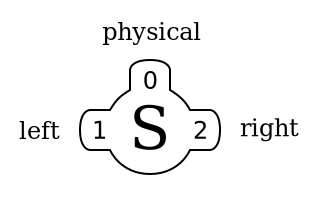
\includegraphics[width=2in]{drawings/state_site_tensor-car}
\end{subfigure}
\begin{subfigure}{2in}
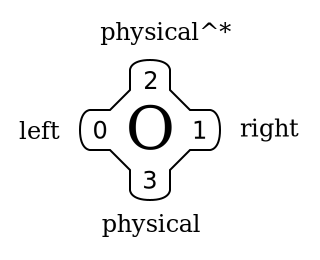
\includegraphics[width=2in]{drawings/operator_site_tensor-car}
\end{subfigure}
\caption{\label{fig:site-tensors-car} Illustrations of the state and operator site tensors.}
\end{figure}

\begin{figure}\begin{center}
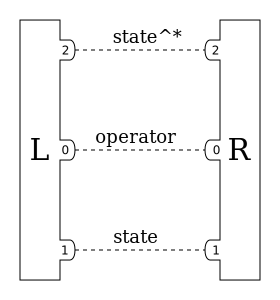
\includegraphics[width=\diagramwidth]{drawings/expectation_boundary_tensors-car}
\caption{\label{fig:environment-tensors-car} Illustration of the environment tensors.}
\end{center}\end{figure}

\begin{figure}\begin{center}
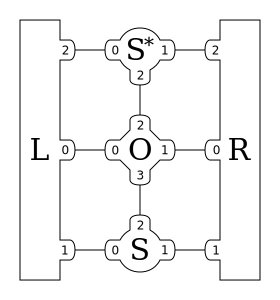
\includegraphics[width=\diagramwidth]{drawings/expectation-car}
\caption{\label{fig:expectation-car} This diagram illustrates the tensor network contraction that obtains the expected value of the observable.  $L$ and $R$ are the environment tensors and $O$ and $S$ are the respective operator and state tensors; $S^*$ denotes the conjugate of $S$.  Note the existence of the following two conventions:  first that the left bandwidth index comes before the right bandwidth index which comes before the physical dimension or dimensions, and that the operator index comes before the state index which comes before the conjugate state index.}
\end{center}\end{figure}

\begin{figure}\begin{center}
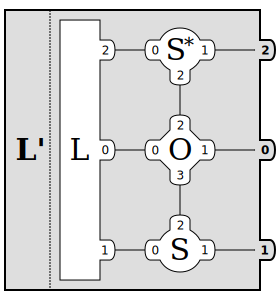
\includegraphics[width=\diagramwidth]{drawings/contractSOSLeft-car}
\caption{\label{fig:contractSOSLeft-car} This diagram illustrates the contraction used to absorb a site into the left environment.}
\end{center}\end{figure}

\begin{figure}\begin{center}
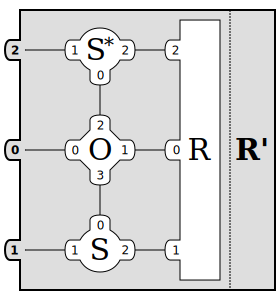
\includegraphics[width=\diagramwidth]{drawings/contractSOSRight-car}
\caption{\label{fig:contractSOSRight-car}This diagram illustrates the contraction used to absorb a site into the right environment.}
\end{center}\end{figure}

\begin{figure}\begin{center}
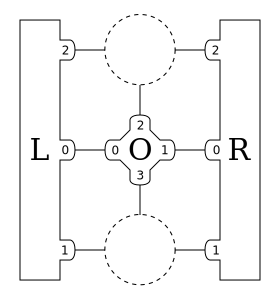
\includegraphics[width=\diagramwidth]{drawings/matmul-car}
\caption{\label{fig:matmul-car}This diagram illustrates how to convert the environment into a matrix.  The bottom hole is where $S$ would normally be and the top hole is where $S^*$ would normally be.  You can use this network for matrix multiplication by inserting $S$ into the bottom hole and then contracting to obtain the result in the top hole.}
\end{center}\end{figure}

\clearpage

\section{The Algorithm}

Conceptually we start with an environment for the operator and an environment for the normalization, but because we assume that our system is in canonical form we can drop the normalization environment (as the norm will always be 1) and so we only need to carry around the operator environment.

The basic idea behind the algorithm is that we start from a trivial representation of the system --- that is where all bond dimensions are set to 1 --- and then grow the bond dimensions until we seem to have converged to a solution.  Thus, we have two levels of iterations:  the higher-level iterates over increasing bond dimensions until they seem to have converged, and the lower level ``sweeps'' by alternating between improving the center site (using an eigensolver) and absorbing it into the left or right environment.  This algorithm is presented in pseudo-code form in Figure \ref{fig:Compute-Ground-State}.

\begin{figure}
\begin{codebox}
\Procname{$\proc{Compute-Ground-State}(O,L^O,R^O,b,t_1,t_2)$}
\li $S \gets$ random tensor with shape $\const{physical-dimension}\times1\times 1$
\li $L \gets L^O$ reshaped to $\text{dim}(L^O)\times1\times1$
\li $R \gets R^O$ reshaped to $\text{dim}(R^O)\times1\times1$
\li $\proc{Sweep-Until-Converged}(S,L,R,O,t_2)$
\li $\id{old\_energy} \gets 0$
\li $\id{new\_energy} \gets  \proc{Compute-Energy(S,L,R,O)}$
\li \While $|old\_energy-new\_energy| \ge t_1$
\li     \Do
\li         $\id{old\_energy} \gets \id{new\_energy}$
\li         $\proc{Increase-Bandwidth}(b,S,L,R)$
\li         $\proc{Sweep-Until-Converged}(S,L,R,t_2,t_3)$
\End
\li return $S,L,R$
\end{codebox}
\caption{\label{fig:Compute-Ground-State} This function finds the minimal eigenstate for the given matrix product operator.  Here $O$ is the matrix product operator site tensor, $L^O$ and $R^O$ are respectively the left and right boundaries for the operator, $b$ is a function that computes how much to raise the bandwidth dimension by, and $t_1$ and $t_2$ are the thresholds used to gauge whether we have converged respectively after increasing the bandwidth dimension and after making a left-right ``sweep''.  This procedure works by repeatedly increasing the bandwidth and converging to the minimal state given that bandwidth until the difference in the eigenvalue between the old (less bandwidth) state and the new (greater bandwidth) state is below $t_1$, at which point victory is delcared. This procedure depends on \proc{Sweep-Until-Converged} to performs sweeps, which is listed in Figure \ref{fig:Sweep-Until-Converged}.}
\end{figure}

\begin{figure}
\begin{codebox}
\Procname{$\proc{Sweep-Until-Converged}(S,L,R,O,t)$}
\li $\id{old\_energy} \gets 0$
\li $\proc{Perform-Sweep}(S,L,R,O)$
\li \While $|old\_energy-new\_energy| \ge t$
\li     \Do
\li         $\id{old\_energy} \gets \id{new\_energy}$
\li         $\proc{Perform-Sweep}(S,L,R,O)$
\li         $\id{new\_energy} \gets  \proc{Compute-Energy(S,L,R,O)}$
\end{codebox}
\caption{\label{fig:Sweep-Until-Converged} This function performs sweeps until the state has converged. Here $S$ is the state site tensor, $O$ is the operator site tensor, $L$ and $R$ respectively the left and right operator environments, and $t$ is the threshold that determines when the sweeping has converged; i.e. the state will be declared to have been converged when, after a sweep, the difference between the old value and the new value is below $t$.  This procedure depends on \proc{Perform-Sweep}, which is listed in Figure \ref{fig:Perform-Sweep}}
\end{figure}

\begin{figure}
\begin{codebox}
\Procname{$\proc{Perform-Sweep}(S,L,R,O)$}
\li $\proc{Improve-Site}(S,L,R,O)$
\li $\proc{Absorb}(0,L,S,O)$
\li $\proc{Improve-Site}(S,L,R,O)$
\li $\proc{Absorb}(1,R,S,O)$
\end{codebox}
\caption{\label{fig:Perform-Sweep} This function performs two iterations that each consist of improving the site and then absorbing it between either the left or right.  Here $S$ is the state site tensor, $O$ is the operator site tensor, and $L$ and $R$ respectively the left and right operator environments.  \proc{Improve-Site} is }
\end{figure}

The \proc{Absorb-Left} and \proc{Absorb-Right} functions are implementations of the tensor contractions illustrated in respectively Figures \ref{fig:contractSOSLeft-car} and \ref{fig:contractSOSRight-car}.

\begin{figure}
\begin{codebox}
\Procname{$\proc{Improve-Site}(S,L,R,O)$}
\li Define the function \id{matmul} to be the matrix multiplication operation
\zi illustrated in Figure \ref{fig:matmul-car}.
\li Invoke ARPACK requesting the minimum eignevalue an associated,
\zi eigenvector with \id{matmul} for the matrix multiplication function and
\zi $S$ for the initial guess.
\li $S \gets$ the new minimal eigenvector
\end{codebox}
\caption{This procedure finds the state site tensor that minimizes the expectation value of the tensor network illustrated in Figure \ref{fig:expectation-car}. Here $S$ is the state site tensor, $O$ is the operator site tensor, and $L$ and $R$ respectively the left and right operator environments.}
\end{figure}

\part{2D Simulation Algorithm}
\label{2dsim}

\part{Appendix}

\begin{appendices}
\section{Optimal Contractions for 1D}
\label{apndx:optimal-contractions}

The tensor contractions in this appendix are ones that have been optimized for efficiency by experimenting with different choices for the index and contraction ordering.  The optimized site tensors are in Figure \ref{fig:site-tensors-opt}, and the optimized environment tensors are in Figure \ref{fig:environment-tensors-opt}.  The expectation value tensor network is in Figure \ref{fig:expectation-opt}.  The optimized subroutines for absorbing the site the left and right environments are shown in respectively Figures \ref{fig:contract_sos_left-opt} and \ref{fig:contract_sos_right-opt}, and the optimized routine for performing matrix multiplication for ARPACK is illustrated in Figure \ref{fig:iteration-opt}.

\begin{figure}
\centering
\begin{subfigure}{2in}
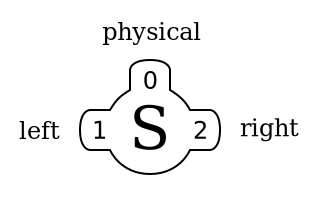
\includegraphics[width=2in]{drawings/state_site_tensor-car}
\end{subfigure}
\begin{subfigure}{2in}
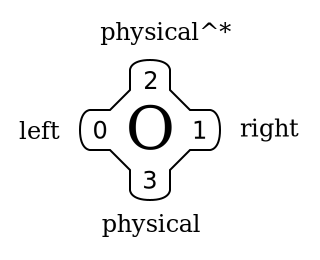
\includegraphics[width=2in]{drawings/operator_site_tensor-car}
\end{subfigure}
\caption{\label{fig:site-tensors-opt} Illustrations of the state and operator site tensors.}
\end{figure}

\begin{figure}\begin{center}
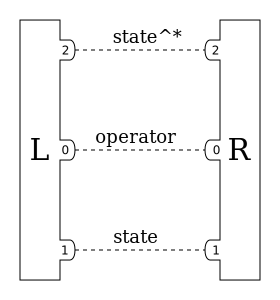
\includegraphics[width=\diagramwidth]{drawings/expectation_boundary_tensors-car}
\caption{\label{fig:environment-tensors-opt} Illustration of the environment tensors.}
\end{center}\end{figure}

\begin{figure}\begin{center}
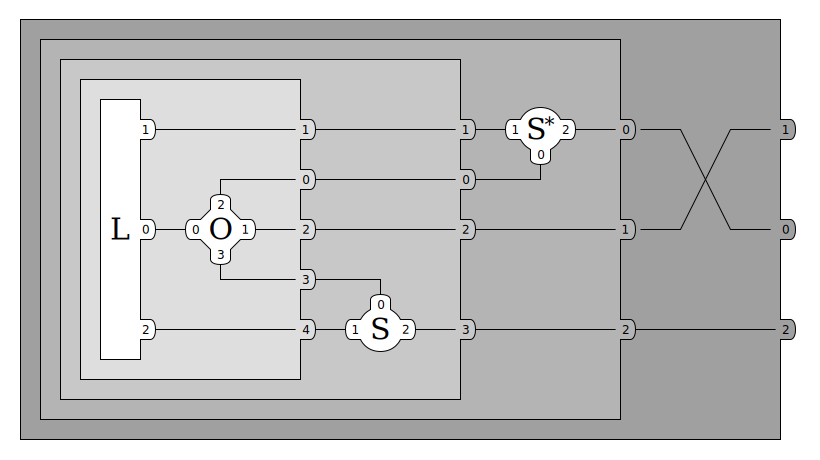
\includegraphics[width=\diagramwidth]{drawings/contract_sos_left-opt}
\caption{\label{fig:contract_sos_left-opt} This diagram illustrates the contraction used to absorb a site into the left environment.}
\end{center}\end{figure}

\begin{figure}\begin{center}
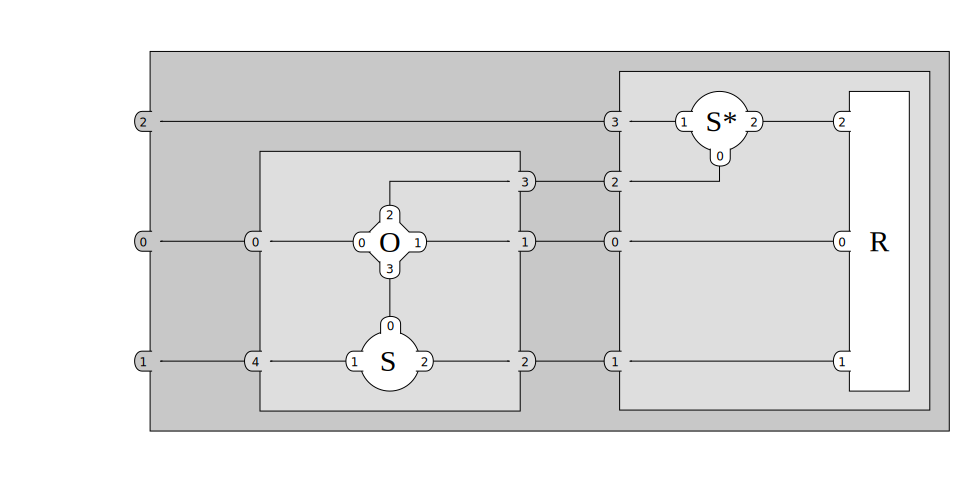
\includegraphics[width=\diagramwidth]{drawings/contract_sos_right-opt}
\caption{\label{fig:contract_sos_right-opt} This diagram illustrates the contraction used to absorb a site into the right environment.}
\end{center}\end{figure}

\begin{figure}\begin{center}
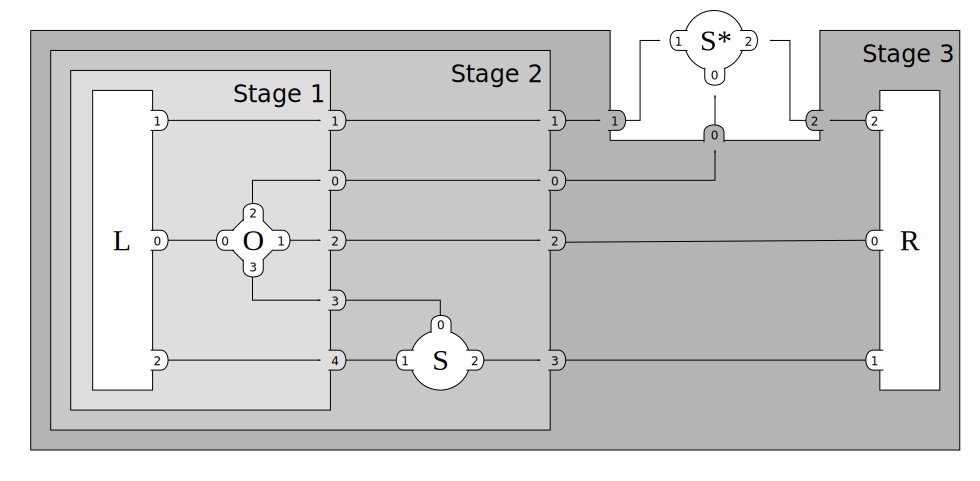
\includegraphics[width=\diagramwidth]{drawings/iteration-opt}
\caption{\label{fig:iteration-opt} This diagram illustrates the contraction used to perform the matrix multiplication used by the ARPACK eigensolver.}
\end{center}\end{figure}

\clearpage

\end{appendices}

\part{Bibliography}

\bibliography{report.bib}
\bibliographystyle{plain}

\end{document}